\documentclass{beamer}

\mode<presentation>{
\usetheme{Madrid}
\setbeamertemplate{navigation symbols}{}
}

\usepackage{graphicx}
\usepackage{booktabs}
\usepackage{tikz}
\usetikzlibrary{spy}

\usepackage[spanish]{babel}
\usepackage[latin1]{inputenc}

%====================================

\title[Trabajo de fin de m�ster]{Redes Generativas Antag�nicas}

\author[Ant�n Makarov]{Ant�n Makarov Samusev}
\institute[UCM/UPM]
{
Universidad Complutense de Madrid \\
Universidad Polit�cnica de Madrid \\
\medskip
\textit{amakarov@ucm.es} \\
\medskip
Dirigido por Francisco Javier Y��ez Gestoso
}
\date{25 de septiembre de 2019}

%====================================

\begin{document}

\begin{frame}
\titlepage
\end{frame}

%====================================

\begin{frame}
\frametitle{�ndice}
\tableofcontents
\end{frame}

%====================================

%------------------------------------------------
\section{Redes Generativas Antag�nicas}
%------------------------------------------------

\begin{frame}
	\frametitle{Descripci�n del problema}
	\begin{itemize}
	\item <1-> Goodfellow et. al. 2014
	\item <2-> Aprendizaje no supervisado
	\item <3-> Describir la distribuci�n que siguen los datos
	\item <4-> Generar muestras a partir de dicha distribuci�n
	\item <5->  Mediante redes neuronales que compiten entre s�
	\end{itemize}
\end{frame}

\begin{frame}
\frametitle{Idea conceptual}
\begin{figure}
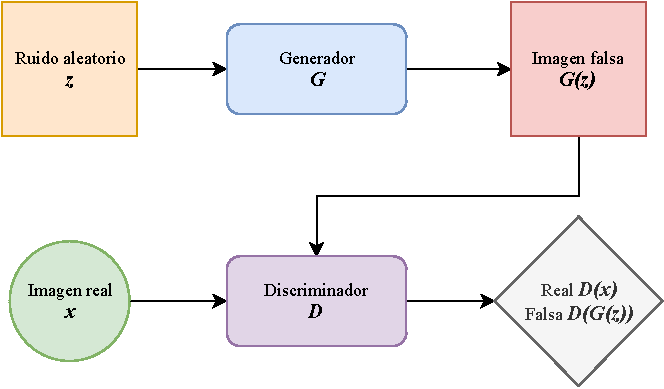
\includegraphics[width=0.8\linewidth]{../images/presentation/scheme.pdf}
\end{figure}
\end{frame}

\begin{frame}
\frametitle{Aspectos te�ricos}
\begin{equation*}
\min_G \max_D V(G,D) = \mathbb{E}_{x \sim p_d(x)} [\log D(x)] + \mathbb{E}_{z \sim p_z(z)} [\log (1- D(G(z)))].
\label{minimax}
\end{equation*}
\end{frame}

%------------------------------------------------
\section{Generaci�n de arte}
\subsection{Redes neuronales convolucionales}
%------------------------------------------------

\begin{frame}
	\frametitle{CNN I}
	\begin{figure}
		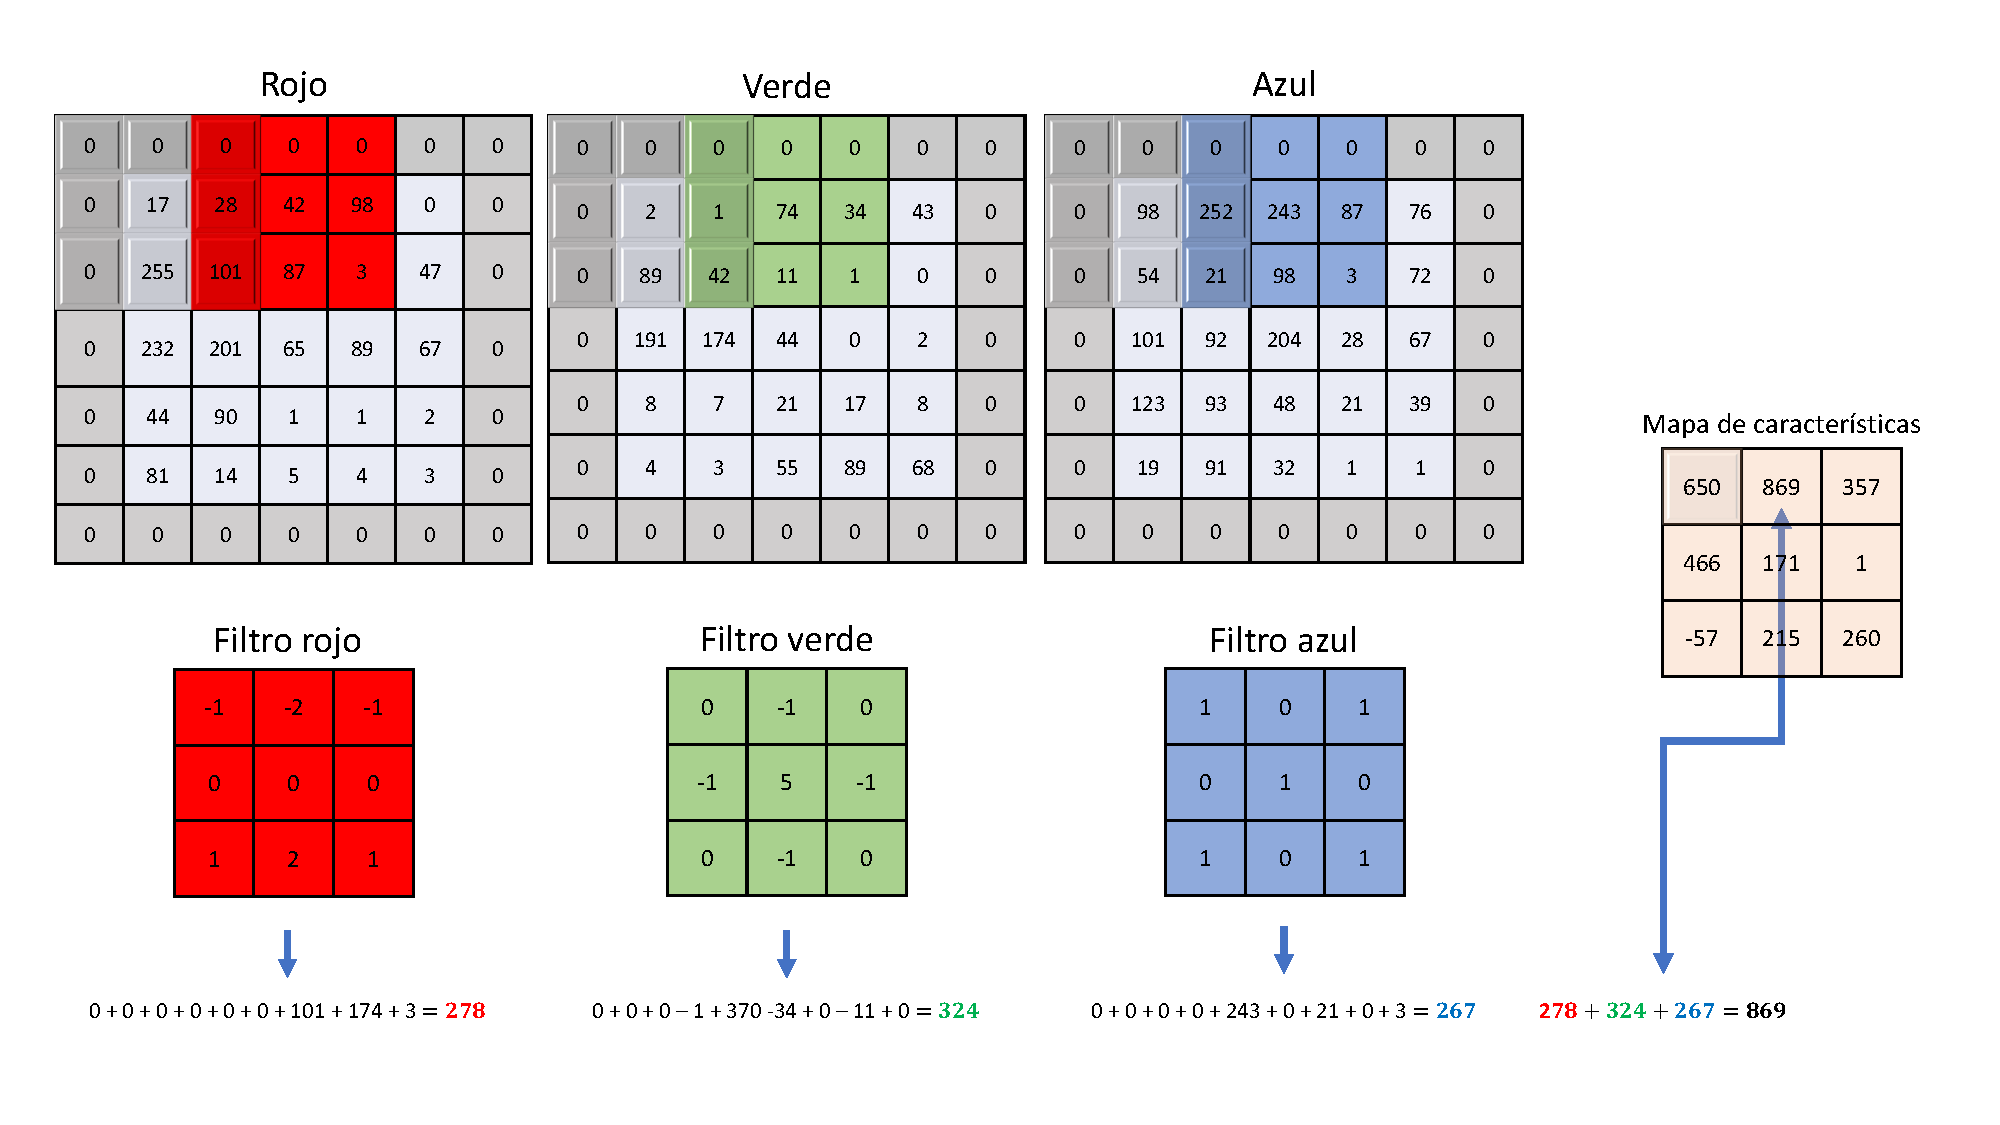
\includegraphics[width=1\linewidth]{../images/presentation/convolut.pdf}
	\end{figure}
\end{frame}

\begin{frame}
	\frametitle{CNN II}
	\begin{figure}
		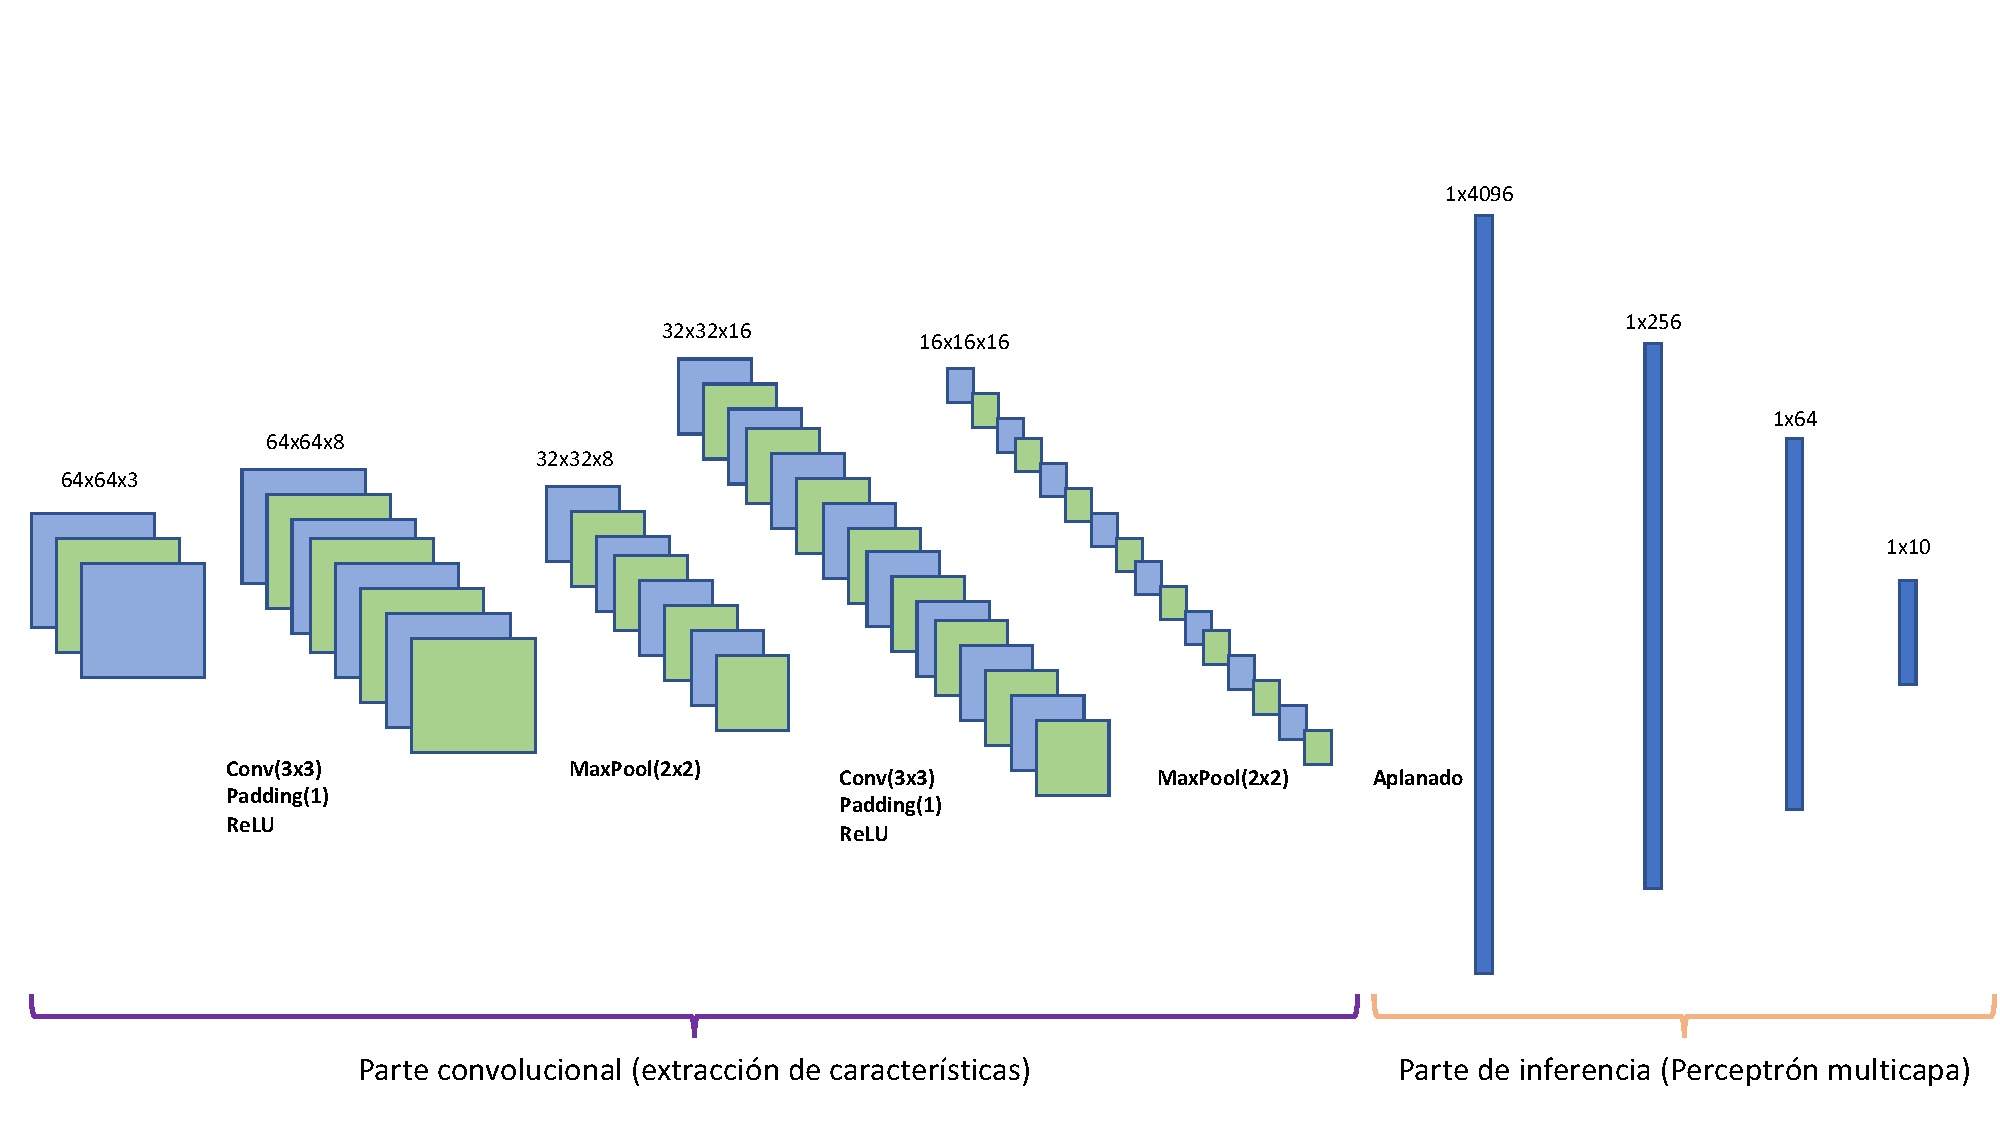
\includegraphics[width=1\linewidth]{../images/presentation/red.pdf}
	\end{figure}
\end{frame}


%------------------------------------------------
\subsection{DCGAN}
%------------------------------------------------

\begin{frame}
\frametitle{DCGAN}
\center \textbf{Deep Convolutional Generative Adversarial Network}
\vfill
\begin{itemize}
	\item Discriminador: Convoluci�n con stride
	\item Generador: Convoluci�n fraccional con stride
	\item No utilizar capas totalmente conectadas
	\item Generador: ReLU $+ \tanh$
	\item Discriminador: LeakyReLU $+$ sigmoide
	\item BatchNorm
	\item Inicializaci�n gaussiana
	\item <2-> One sided label smoothing
\end{itemize}
\huge \uncover<3->{\url{https://github.com/ant-mak/tfm}}
\end{frame}

%------------------------------------------------
\subsection{Metodolog�a}
%------------------------------------------------

\begin{frame}
\frametitle{Obtenci�n y pre-procesado}
	\begin{itemize}
		\item Conjunto de datos obtenido de una competici�n de Kaggle
		\item M�s de 100000 im�genes $\approx 50$ GB
		\item Algunas im�genes corruptas
		\item Escalado de tama�os y proporciones
		\item Normalizaci�n
		\item Carga como tensores
	\end{itemize}
\end{frame}

\begin{frame}
	\begin{figure}
		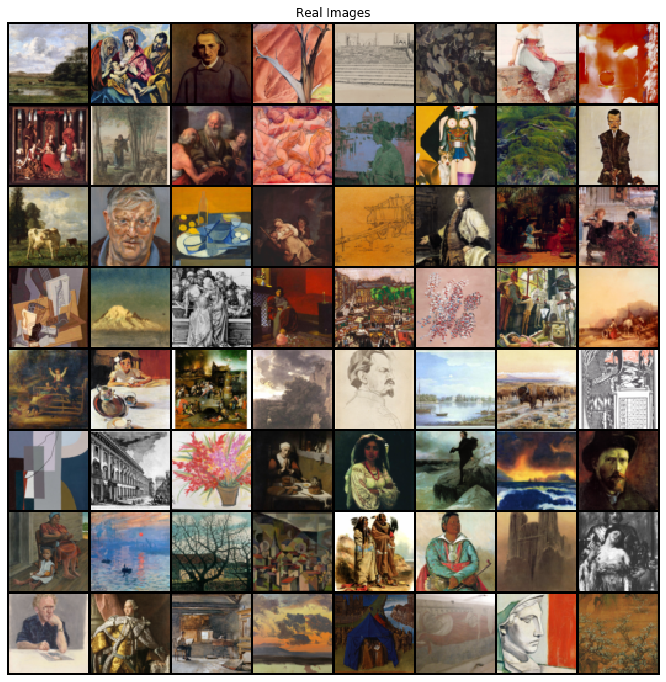
\includegraphics[width=0.7\linewidth]{../images/results/original_data.png}
	\end{figure}
\end{frame}

\begin{frame}
\begin{tikzpicture}[spy using outlines={magnification=3,size=5cm, connect spies}]

\node {\pgfimage[interpolate=true,width=0.5\linewidth]{../images/presentation/architecture.pdf}};
\only<1>\spy on (-1.98,1) in node [left] at (-4,1);
\only<2>\spy on (1.93,1.5) in node [left] at (-4,1);
\end{tikzpicture}
\end{frame}

%------------------------------------------------
\subsection{Recursos y rendimiento}
%------------------------------------------------

\begin{frame}
	\frametitle{Recursos y rendimiento}
	\begin{itemize}
		\item Imprescindible GPU para el entrenamiento
		\item 24 horas para 30 �pocas
		\item en PC normal, 20 veces m�s lento
	\end{itemize}
\end{frame}

%------------------------------------------------
\subsection{Resultados}
%------------------------------------------------

\begin{frame}
	\begin{figure}
		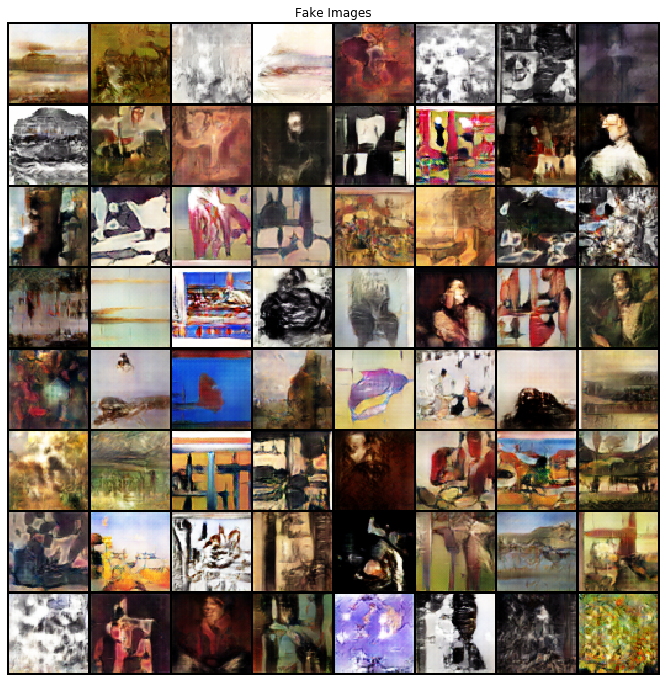
\includegraphics[width=0.7\linewidth]{../images/results/generated_data.png}
	\end{figure}
\end{frame}

\begin{frame}
	\begin{figure}
	\includegraphics<1>[width=0.8\linewidth]{../images/presentation/ev-0.png}
	\includegraphics<2>[width=0.8\linewidth]{../images/presentation/ev-1.png}
	\includegraphics<3>[width=0.8\linewidth]{../images/presentation/ev-2.png}
	\includegraphics<4>[width=0.8\linewidth]{../images/presentation/ev-3.png}
	\includegraphics<5>[width=0.8\linewidth]{../images/presentation/ev-4.png}
	\includegraphics<6>[width=0.8\linewidth]{../images/presentation/ev-5.png}
	\includegraphics<7>[width=0.8\linewidth]{../images/presentation/ev-6.png}
	\includegraphics<8>[width=0.8\linewidth]{../images/presentation/ev-7.png}
	\end{figure}
\end{frame}

%------------------------------------------------
\section{Algunas arquitecturas basadas en GANs}
%------------------------------------------------

\begin{frame}
	\frametitle{Evoluci�n en generaci�n de caras}
	\begin{figure}
		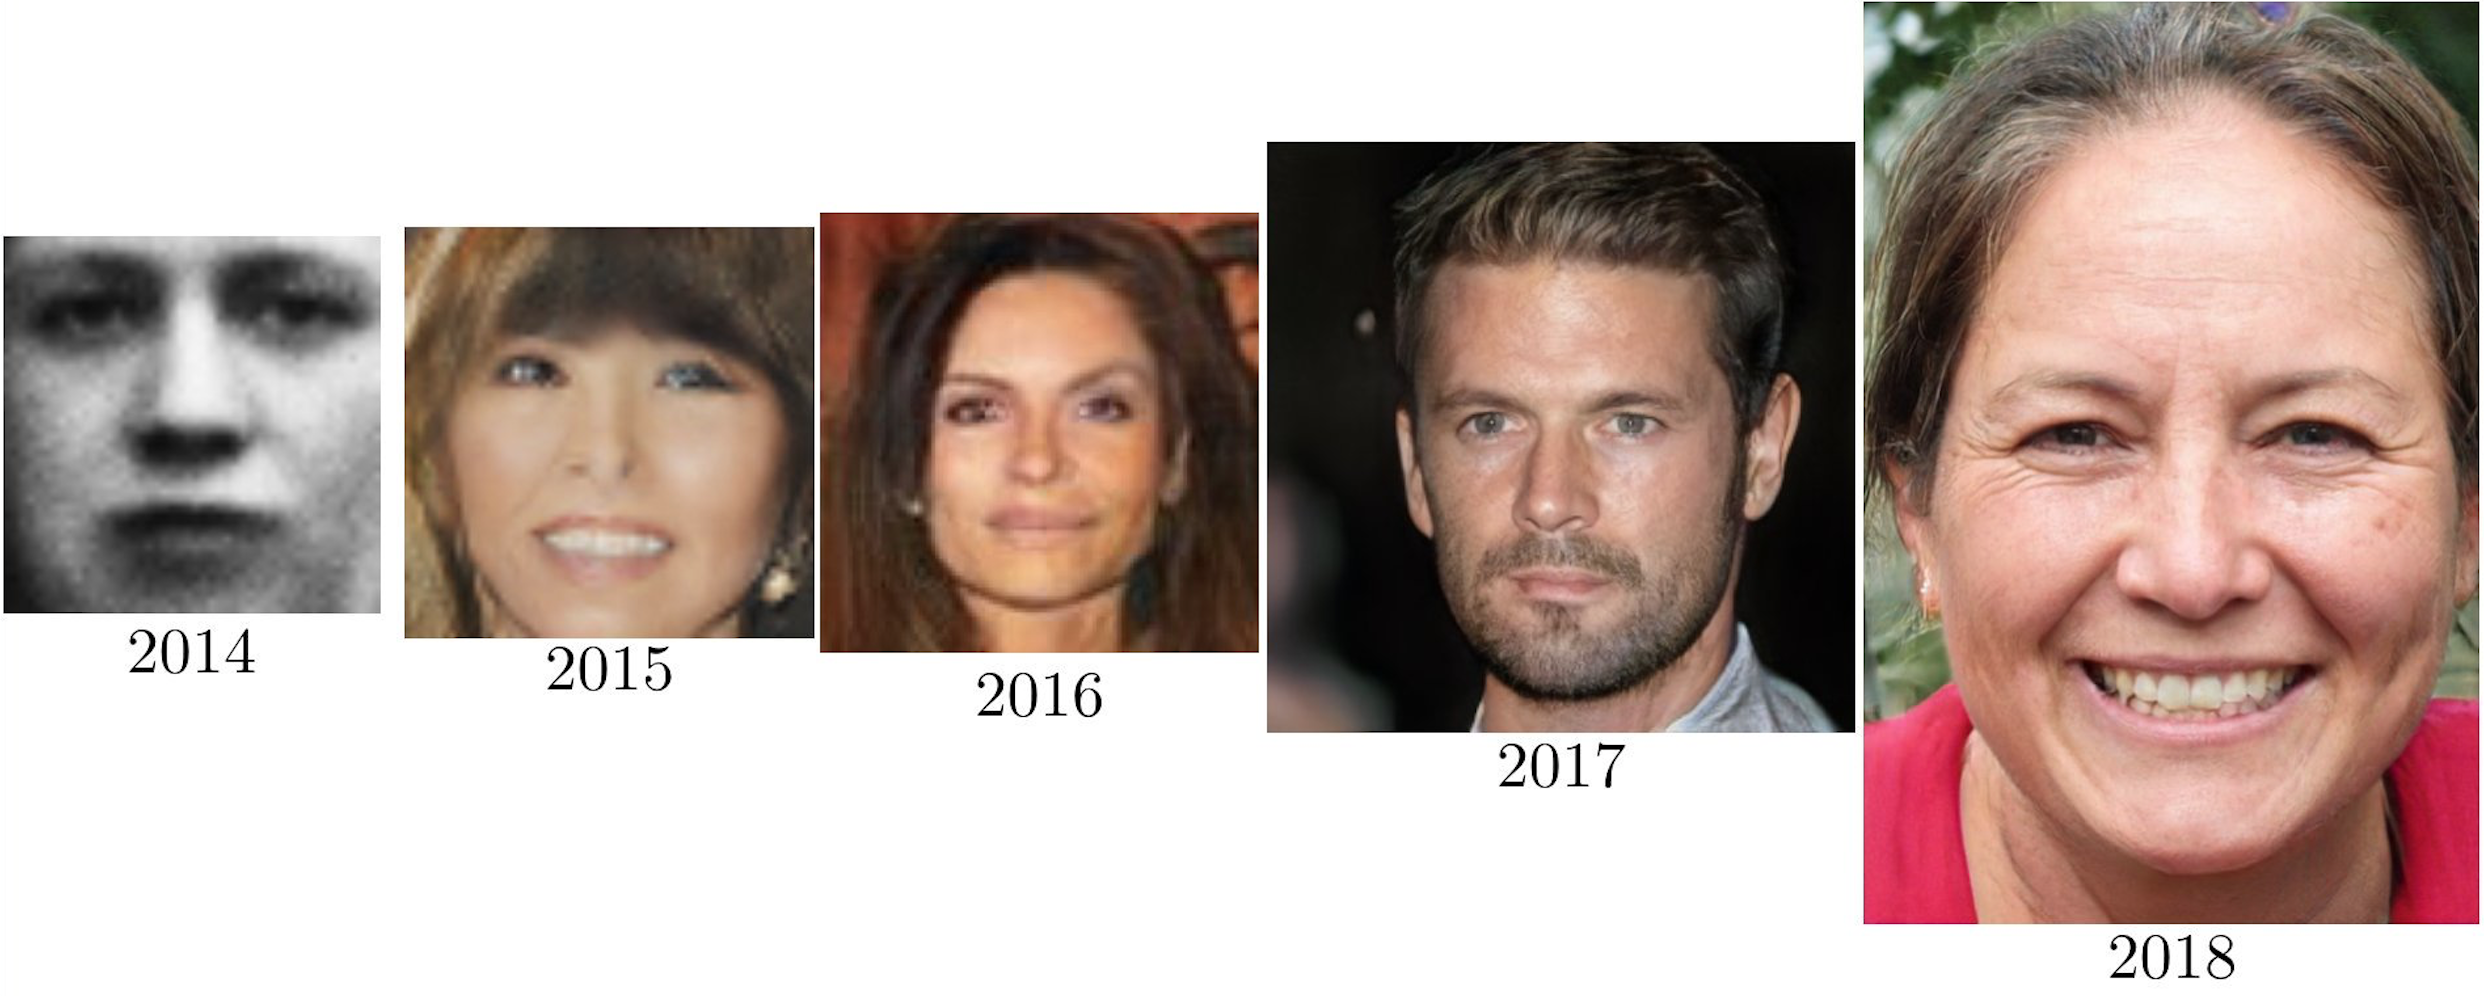
\includegraphics[width=1\linewidth]{../images/presentation/evolution.png}
	\end{figure}
\end{frame}

\begin{frame}
	\frametitle{DCGAN}
	\begin{figure}
		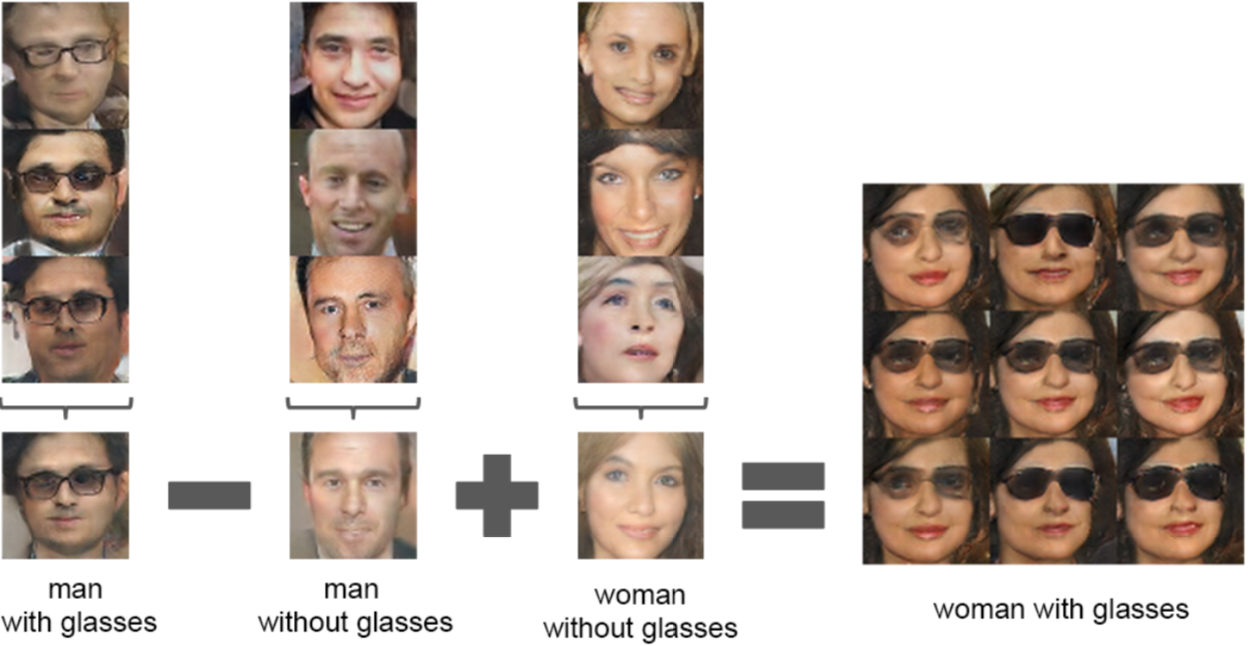
\includegraphics[width=1\linewidth]{../images/presentation/dcgan.png}
	\end{figure}
\end{frame}

\begin{frame}
	\frametitle{Text to image}
	\begin{figure}
		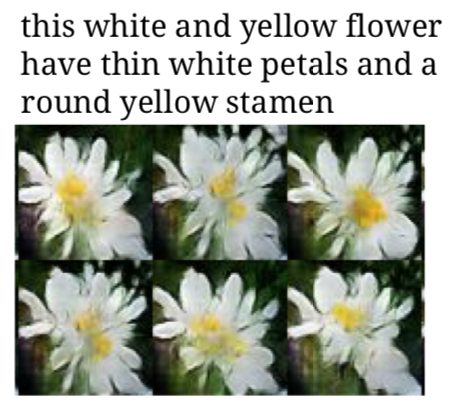
\includegraphics[width=0.7\linewidth]{../images/presentation/text_to_image.png}
	\end{figure}
\end{frame}

\begin{frame}
	\frametitle{PGAN}
	\begin{figure}
		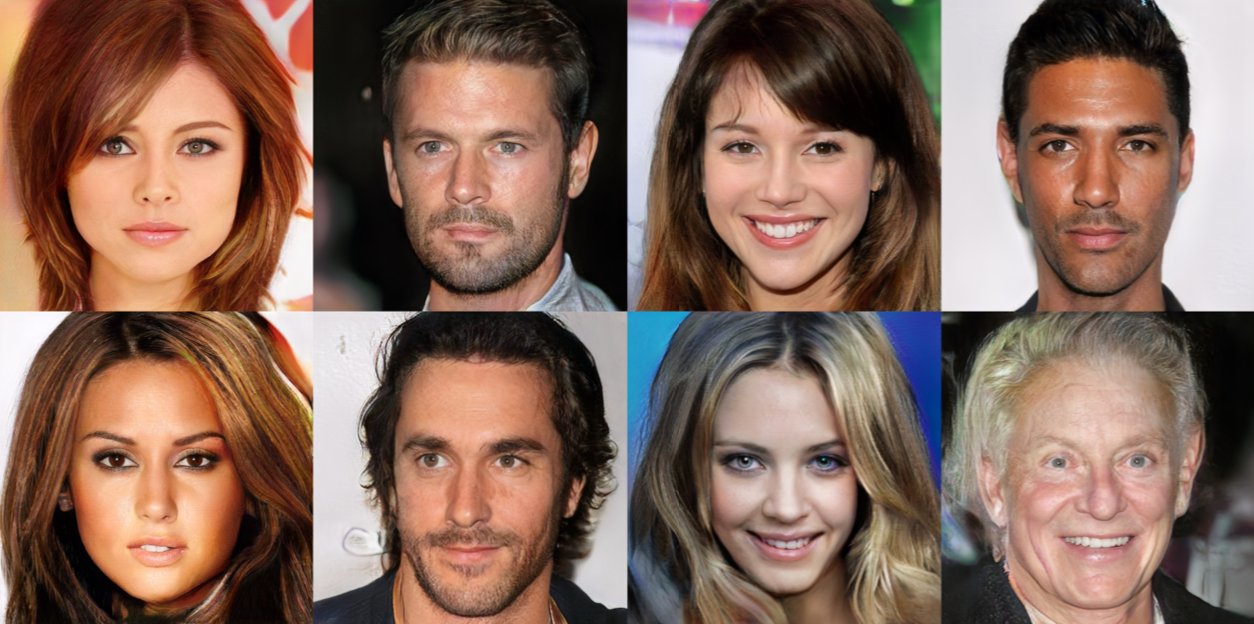
\includegraphics[width=1\linewidth]{../images/presentation/progan.png}
	\end{figure}
\end{frame}

\begin{frame}
	\frametitle{Pix2Pix}
	\begin{figure}
		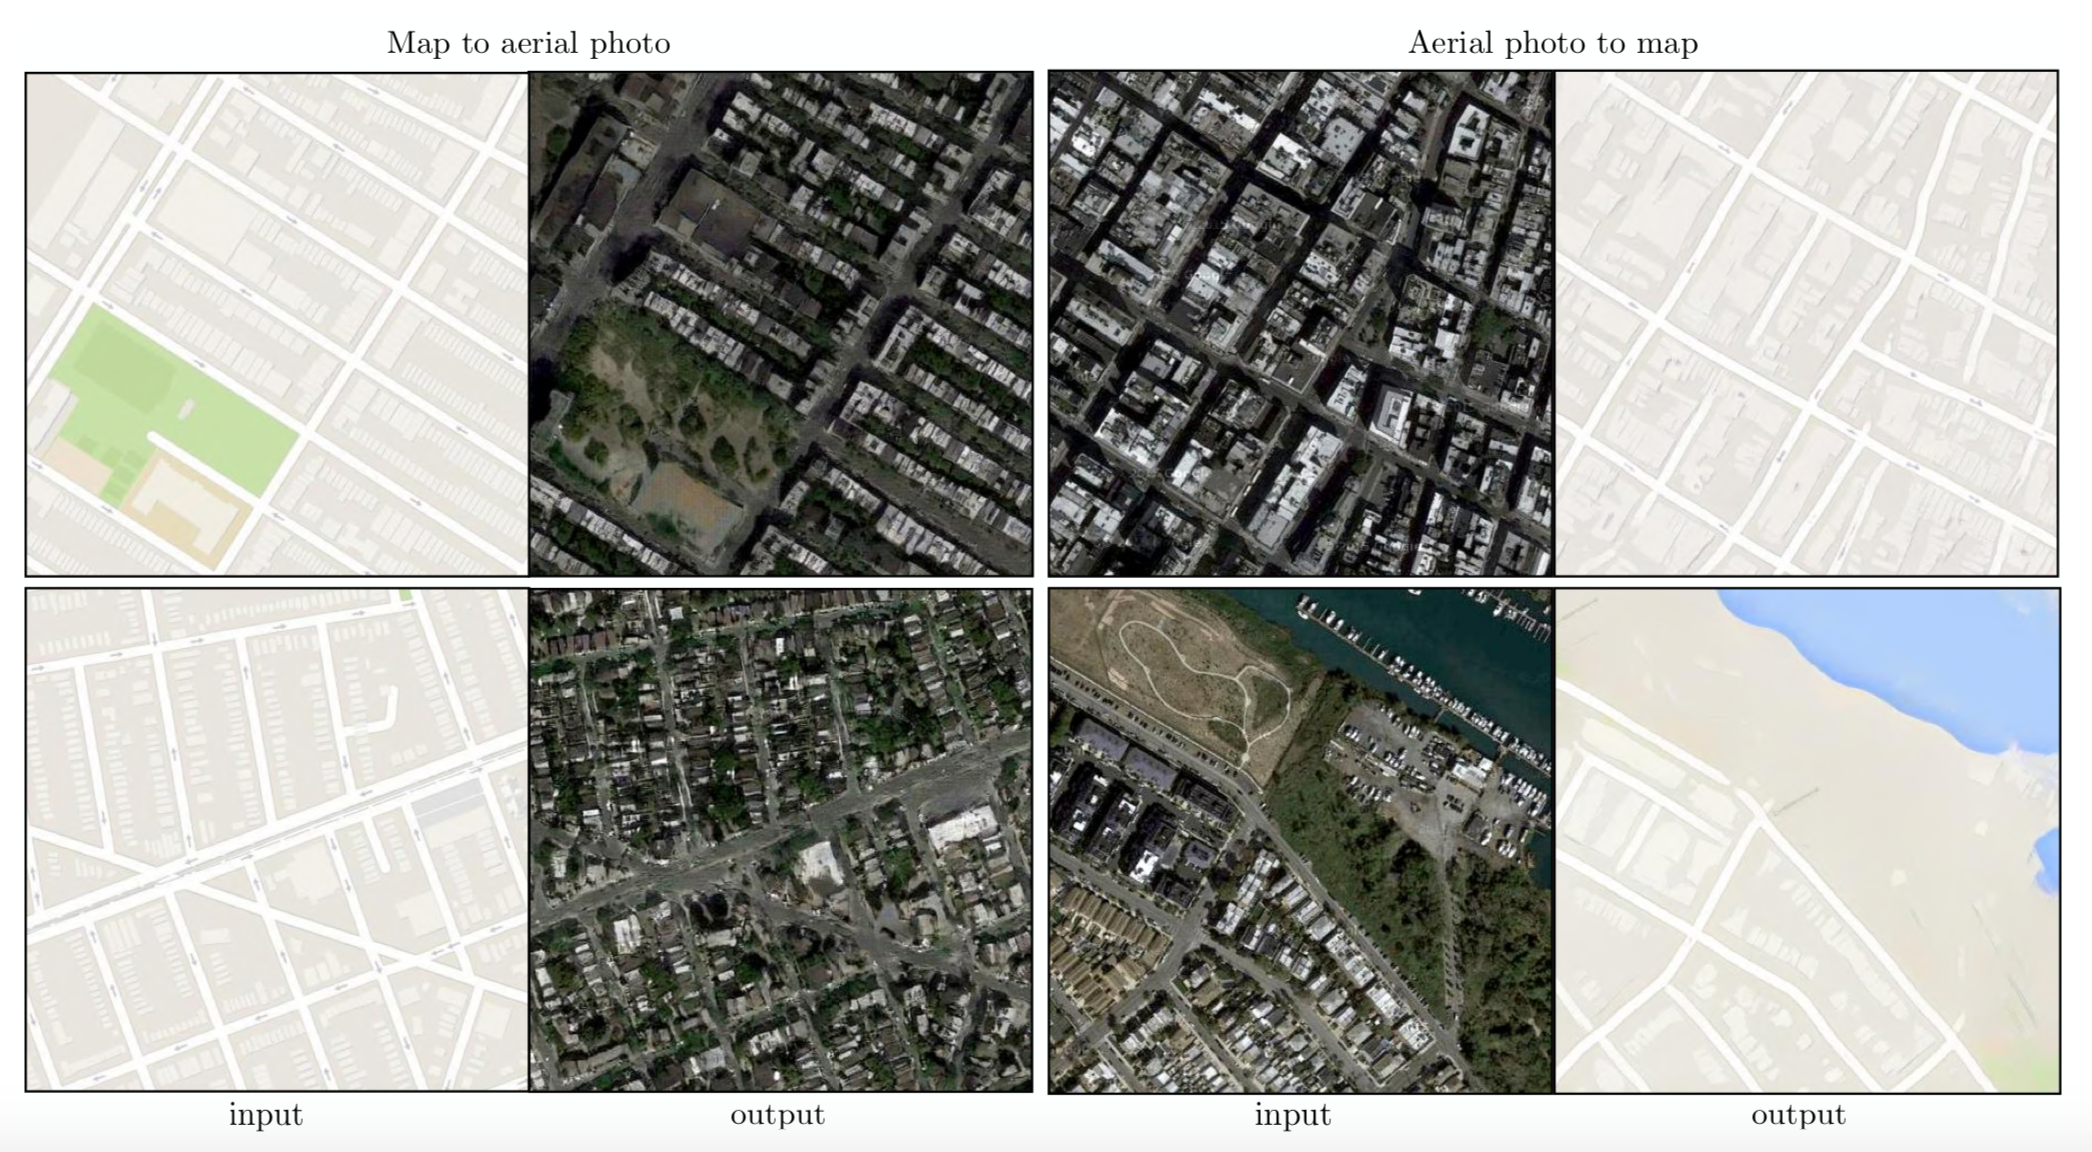
\includegraphics[width=1\linewidth]{../images/presentation/pix2pix.png}
	\end{figure}
\end{frame}

\begin{frame}
	\frametitle{CycleGAN}
	\begin{figure}
		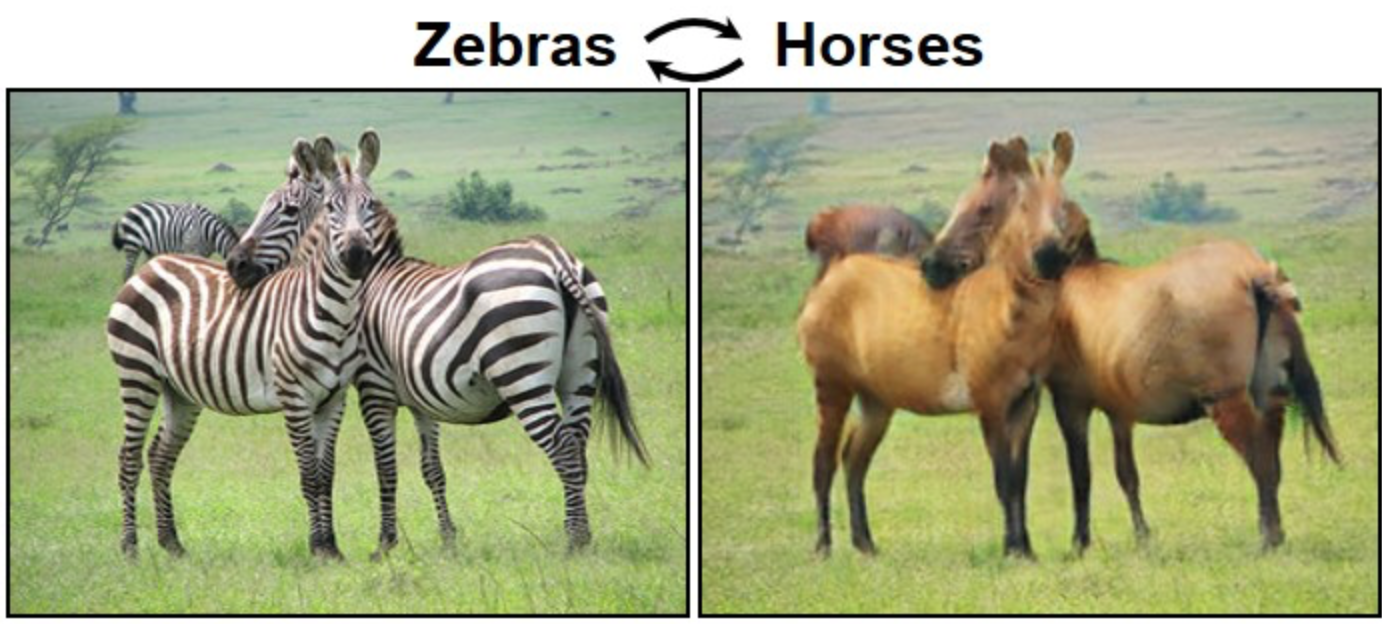
\includegraphics[width=1\linewidth]{../images/presentation/cyclegan.png}
	\end{figure}
\end{frame}

%------------------------------------------------
\section{Consideraciones pr�cticas}
%------------------------------------------------

\begin{frame}
	\frametitle{Consideraciones pr�cticas}
	\begin{itemize}
		\item �C�mo evaluar los resultados?
		\item �C�mo comparar arquitecturas?
		\item Mode collapse
	\end{itemize}
\end{frame}

%------------------------------------------------
\section{Conclusi�n}
%------------------------------------------------

\begin{frame}
\frametitle{Conclusi�n}
\begin{itemize}
	\item Campo de investigaci�n en auge
	\item Interesantes aplicaciones en diversos �mbitos
	\item Dif�cil entrenamiento
	\item Dif�cil evaluaci�n
	\item Consumo de grandes cantidades de recursos computacionales
	\item �A�n quedan muchas cosas por descubrir!
\end{itemize}
\end{frame}

%------------------------------------------------
\section{Referencias principales}
%------------------------------------------------

\begin{frame}
\frametitle{Referencias principales}
\begin{thebibliography}{9}
\bibitem{gan}
I. Goodfellow, J. Pouget-Abadie, M. Mirza, B. Xu, D. Warde-Farley, S. Ozair, A. Courville, and Y. Bengio. Generative adversarial nets. In \textit{Advances in neural information processing systems}, pages 2672--2680, 2014.

\bibitem{dcgan}
A. Radford, L. Metz, and S. Chintala. Unsupervised representation learning with deep convolutional generative adversarial networks. \textit{arXiv preprint arXiv:1511.06434}, 2015.

\bibitem{dl}
I. Goodfellow, Y. Bengio, and A. Courville. \textit{Deep Learning}. MIT Press, 2016. \texttt{http://www.deeplearningbook.org}.

\end{thebibliography}
\end{frame}

%------------------------------------------------

\begin{frame}
\centering
\Huge
Gracias por su atenci�n
\end{frame}

\end{document}